\chapter{ကားရဲလ်နှင့် ရီကားဆစ်ဖ် ဖန်ရှင်များ}

ဖန်ရှင်တစ်ခုကနေ ‘အခြား’ ဖန်ရှင်တွေ ခေါ်သုံးတာကို အခန်း (၃) မှာ တွေ့ခဲ့ပြီးပါပြီ။ ဒါပေမဲ့ ဖန်ရှင်တစ်ခုက ၎င်းကိုယ်၎င်း ပြန်ခေါ်ထားတာကိုတော့ မကြုံဖူးသေးပါဘူး။ ဖန်ရှင်တွေဟာ ဆော့ဖ်ဝဲ အဆောက်အဦး တည်ဆောက်ရာမှာ မရှိမဖြစ်တဲ့ အခြေခံအုတ်ချပ်တွေလို့ ဆိုရမှာပါ။  ၎င်းကိုယ်တိုင်ကို ပြန်လည်အသုံးပြု၍ ဖန်ရှင်အုတ်ချပ်တစ်ခု ဖန်တီးလို့ ရနိုင်ပါမလား။ ဒီမေးခွန်းဟာ  ထူးဆန်းကောင်း ထူးဆန်းနေပါလိမ့်မယ်။ အခြေခံကျပြီး စိတ်ဝင်စားစရာကောင်းတဲ့ ဖီလော်ဆော်ဖီ မေးခွန်းလည်း ဖြစ်တယ်။

%\fEn{Recursive function} တွေဟာ  ခေါ် ဂျန်နရယ် ကွန်းဆက်ပ်မှာ အကျုံးဝင်တဲ့ ဥပမာတစ်ခုသာ ဖြစ်တယ်။ \fEnEmp{Recursion} ဆိုတာ 

%\fEnEmp{Recursion} ကတော့ ပိုပြီး ကျယ်ပြန့်တဲ့၊ ဂျန်နရယ်ကျတဲ့ ကွန်းဆက်ပ်ကို ရည်ညွှန်း‌ ဖော်ပြတာ ဖြစ်တယ်။ ရုပ်ပုံတစ်ခုမှာ \fEnEmp{recursion} သဘောတရား ပါဝင်နေရင် \fEn{recursive shape} ၊ ဖြစ်စဉ်တစ်ခုမှာ \fEnEmp{recursion} သဘောတရား ပါဝင်နေရင် \fEn{recursive process} ၊ အဓိပ္ပါယ်

ဖန်ရှင် သတ်မှတ်ချက်ထဲမှာ ၎င်းဖန်ရှင်ကိုယ်တိုင်ကို ပြန်ခေါ်လို့ ရပါတယ်။ ရီကားဆစ်ဖ် ဖန်ရှင် \fEn{(\textit{recursive function})} လို့ ခေါ်တယ်။ ရီကားဆစ်ဖ် ဖန်ရှင်တွေဟာ ဘီဂင်နာ ပရိုဂရမ်မာအတွက် နားလည်ဖို့ ခက်ခဲတဲ့ သဘောတရားအဖြစ် ယူဆကြတာကြောင့် စာအုပ် အတော်များများမှာ  နောက်ကျပြီး ဖော်ပြလေ့ရှိတယ်။ တကယ်က လူများစု ထင်/ပြောသလို နားမလည်နိုင်လောက်အောင် ရှုပ်ထွေး ခက်ခဲတဲ့ သဘောတရား မဟုတ်ပါဘူး။ သာမန်လူအားလုံး နားလည်နိုင်ပါတယ်။ ဒါကြောင့် စောစောစီးစီး အခုပဲ မိတ်ဆက်ပေးလိုက်ပါတယ်။ အကယ်၍ နားမလည်ခဲ့ရင်လည်း ပြဿနာမရှိပါဘူး။ အကြမ်းဖျဉ်းလောက် ဖတ်ကြည့်ပြီး နောက်လာမဲ့ အခန်းတွေကို ကျော်သွားနိုင်ပါတယ်။ နောင်တစ်ချိန်ကျမှ ပြန်လာဖတ်ပေါ့။

\section{ရီကားဆစ်ဖ် ဖန်ရှင် ဘယ်လို အလုပ်လုပ်လဲ}
 ရီကားဆစ်ဖ် ဖန်ရှင် ဥပမာတစ်ခုကို လေ့လာကြည့်ပါမယ်။ အောက်ဖော်ပြပါ ဖန်ရှင်ဟာ \fEnEmp{recursive call} လို့ ကွန်းမန့်ရေးထားတဲ့ လိုင်းမှာ သူ့ကိုယ်သူ ပြန်ခေါ်ထားတာ ဂရုပြုကြည့်ပါ။ 
%
\setlength{\fboxsep}{0pt}
\begin{minted}[frame=\mintframe, framerule=\mintrule,framesep= \mintsep, xleftmargin=\xlftmargin
    , bgcolor=mintbgcolor,rulecolor=mintrulecolor
    , python3=true,escapeinside=ßß]{python}
def make_beeper_row():
    if front_is_clear():
        put_beeper()
        move()
        make_beeper_row() # ß\fEn{recursive call}ß
    else:
        put_beeper()
\end{minted}
%

ဒီဖန်ရှင်ကို ခေါ်လိုက်ရင် ဘာဆက်ဖြစ်မလဲဆိုတာ စိတ်ဝင်စားစရာပါ။  ဖန်ရှင်မစတင်မီ အနေအထားကို ပုံ  (\fRefNo{\ref{fig:mrofb_recur1}}) မှာ ကြည့်ပါ။ ဖန်ရှင်ကို ကနဦး  စခေါ်လိုက်တာမို့လို့ \fEnEmp{initial call} လို့ ရည်ညွှန်းပါမယ်။
%
\setlength{\fboxsep}{0pt}
\begin{minted}[frame=\mintframe, framerule=\mintrule,framesep= \mintsep, xleftmargin=\xlftmargin
    , bgcolor=mintbgcolor,rulecolor=mintrulecolor
    , python3=true,escapeinside=ßß]{python}
# ß\fEn{initial call}ß
make_beeper_row()
\end{minted}
%
\begin{figure}[htb!]
    {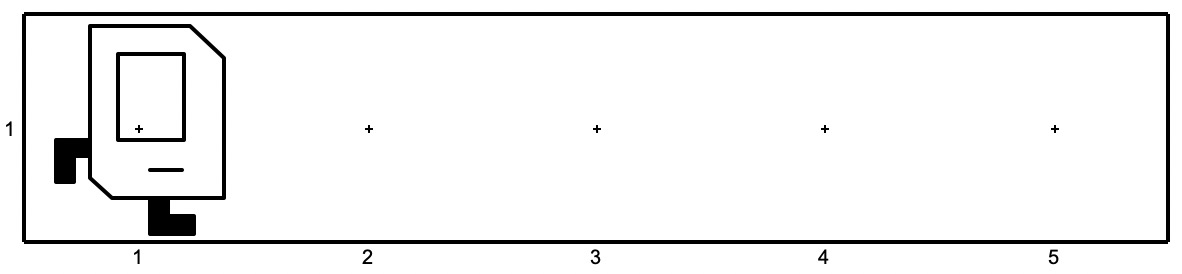
\includegraphics[scale=0.15]{images/ch04/mrofb/before.jpg}}
\caption{}
\label{fig:mrofb_recur1}
\end{figure}

ဖန်ရှင် စတင် လုပ်ဆောင်ပါမယ်။  ရှေ့မှာရှင်းနေတဲ့ အတွက် \fCode{if} ဘလောက်ကို လုပ်မှာပါ
%
\setlength{\fboxsep}{0pt}
\begin{minted}[frame=\mintframe, framerule=\mintrule,framesep= \mintsep, xleftmargin=\xlftmargin
    , bgcolor=mintbgcolor,rulecolor=mintrulecolor
    , python3=true,escapeinside=ßß]{python}
put_beeper()
move()
make_beeper_row() # ß\fEn{recursive call}ß
\end{minted}
%
ဘိပါချ၊ ရှေ့တိုး $\big\llbracket$ပုံ (\fRefNo{\ref{fig:mrofb_recur}}) (\fRefNo{\subref{fig:mrofb_recur2}})  ကြည့်ပါ$\big\rrbracket$ ပြီးရင် သူ့ကိုယ်သူ  ပြန်ခေါ်ထားတယ်။ ဒါဟာ ပထမဆုံး တစ်ကြိမ်ပါ။ ဖန်ရှင်ခေါ်ရင် ဖြစ်မြဲအတိုင်းပဲ ဖန်ရှင်နဲ့ သက်ဆိုင်တဲ့ ဘလောက်ကို ဆောက်ရွက်တာပေါ့။ ဒီတော့ \fCode{make\_beeper\_row} ဖန်ရှင်ဘလောက်ကိုပဲ တစ်ခါထပ်လုပ်မှာပါ။ ရှေ့မှာ ရှင်းနေတဲ့အတွက် \fCode{if} ဘလောက်ကို လုပ်တယ်
%
\setlength{\fboxsep}{0pt}
\begin{minted}[frame=\mintframe, framerule=\mintrule,framesep= \mintsep, xleftmargin=\xlftmargin
    , bgcolor=mintbgcolor,rulecolor=mintrulecolor
    , python3=true,escapeinside=ßß]{python}
put_beeper()
move()
make_beeper_row() # ß\fEn{recursive call}ß
\end{minted}
%
ဘိပါချ၊ ရှေ့တိုး $\big\llbracket$ပုံ (\fRefNo{\ref{fig:mrofb_recur}}) (\fRefNo{\subref{fig:mrofb_recur3}})$\big\rrbracket$ ပြီး သူ့ကိုယ်သူ ပြန်ခေါ်ထားတဲ့ကိစ္စ တစ်ခါထပ်ဖြစ်ပြန်တယ်။ ဒါနဲ့ဆို နှစ်ကြိမ်။ ဖန်ရှင်ဘလောက် အလုပ် ပြန်လုပ်မယ်။ ရှေ့မှာရှင်းတယ်၊ \fCode{if} ဘလောက်ကိုပဲ ထပ်လုပ်
%
\setlength{\fboxsep}{0pt}
\begin{minted}[frame=\mintframe, framerule=\mintrule,framesep= \mintsep, xleftmargin=\xlftmargin
    , bgcolor=mintbgcolor,rulecolor=mintrulecolor
    , python3=true,escapeinside=ßß]{python}
put_beeper()
move()
make_beeper_row() # ß\fEn{recursive call}ß
\end{minted}
%
ပုံ (\fRefNo{\ref{fig:mrofb_recur}}) (\fRefNo{\subref{fig:mrofb_recur4}}) နေရာရောက်ပြီး သူ့ကိုယ်သူ ထပ်ခေါ်ထားပြန်တယ်။ \fCode{if} ဘလောက် ထပ်လုပ်
%
\setlength{\fboxsep}{0pt}
\begin{minted}[frame=\mintframe, framerule=\mintrule,framesep= \mintsep, xleftmargin=\xlftmargin
    , bgcolor=mintbgcolor,rulecolor=mintrulecolor
    , python3=true,escapeinside=ßß]{python}
put_beeper()
move()
make_beeper_row() # ß\fEn{recursive call}ß
\end{minted}
%
ရှေ့တိုးပြီးရင် နံရံပိတ်နေပြီ $\big\llbracket$ပုံ (\fRefNo{\ref{fig:mrofb_recur}}) (\fRefNo{\subref{fig:mrofb_recur5}})$\big\rrbracket$။ သူ့ကိုယ်သူ ခေါ်တယ်။ ရှေ့မှာ ပိတ်နေတဲ့အတွက် \fCode{else} အပိုင်းကို လုပ်မှာပါ။
%
\setlength{\fboxsep}{0pt}
\begin{minted}[frame=\mintframe, framerule=\mintrule,framesep= \mintsep, xleftmargin=\xlftmargin
    , bgcolor=mintbgcolor,rulecolor=mintrulecolor
    , python3=true,escapeinside=ßß]{python}
put_beeper()
\end{minted}
%
သူ့ကိုယ်သူ ပြန်ခေါ်တဲ့ကစ္စ ထပ်မဖြစ်တော့ဘူး။ ဒီမှာပဲ ပြီးဆုံးသွားတယ်။ ရီကားဆစ်ဖ် ဖန်ရှင် အလုပ်လုပ်ပုံ အခြေခံသဘောတရားက ဒါပါပဲ။ \fEn{loop} တွေ မသုံးဘဲ ပြန်ကျော့နေတဲ့ သဘောကို ရီကားဆစ်ဖ်ဖန်ရှင်မှာ တွေ့ရပါတယ်။ ဖန်ရှင်က သူ့ကိုယ်သူ (သို့ ကိုယ့်ကိုကိုယ်) ပြန်ခေါ်တာကို \fEnEmp{recursive call} လို့ခေါ်ပါတယ်။ ဒက်ဖ်နေးရှင်းအရ \fEn{recursive function} တွေမှာ \fEn{recursive call} အနည်းဆုံး တစ်ခု ပါရမှာ ဖြစ်ပါတယ်။


%ဒီတိုင်း ဆက်ကြည့်သွားရင် လေးကြိမ်မြောက် ရီကားဆစ်ဖ်‌ ကောလ်မှာ ရှေ့မှာနံရံပိတ်နေပြီ $\big\llbracket$ပုံ (\fRefNo{\ref{fig:mrofb_recur}}) (\fRefNo{\subref{fig:mrofb_recur4}})$\big\rrbracket$။ ဒီတော့ \fCode{else} အပိုင်း အလုပ်လုပ်ပါမယ်။ နောက်ဆုံး ဘိပါချမယ်။ ရီကားဆစ်ဖ်ကောလ် ဆက်မဖြစ်တော့ဘူး။ ဒီအခါ တစ်ဖက်စာမျက်နှာ \fEnEmpBf{*Initial Call*} ကွန်းမန့်အောက် ကနဦး \fCode{make\_beeper\_row} ဖန်ရှင်ကောလ်ကနေ စတင်ဖြစ်ပေါ်စေတဲ့ ရီးကားဆစ်ဖ်ဖန်ရှင် လုပ်ဆောင်မှုလည်း ပြီးဆုံးသွားမှာဖြစ်တယ်။

\begin{figure}[thb!]
    \newcommand{\figpctw}{0.49}
    \begin{subfigure}[t]{{\figpctw}\textwidth}
        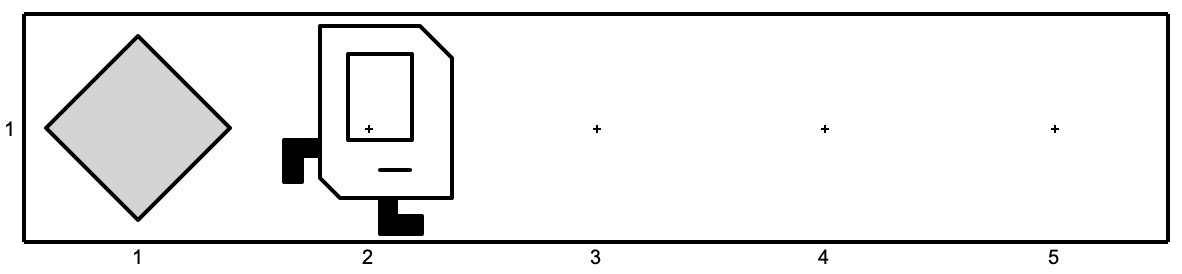
\includegraphics[scale=0.15]{images/ch04/mrofb/1st_iter.jpg}
        \caption{ပထမ တစ်ကျော့ပြီး}  
        \label{fig:mrofb_recur2}   
    \end{subfigure}
    \begin{subfigure}[t]{{\figpctw}\textwidth}
        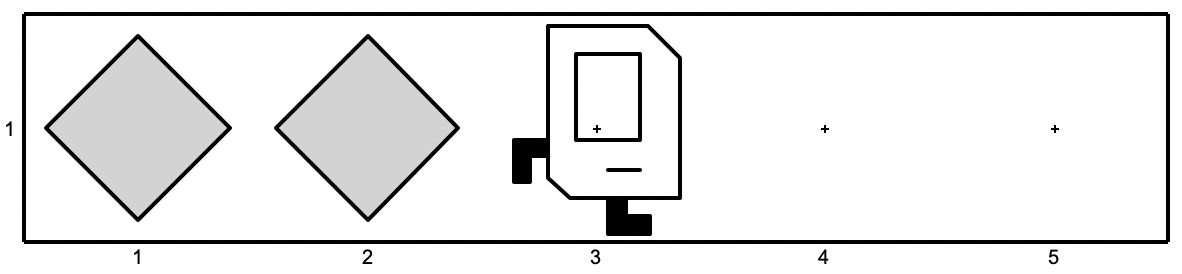
\includegraphics[scale=0.15]{images/ch04/mrofb/2nd_iter.jpg}
        \caption{ဒုတိယ တစ်ကျော့ပြီး}  
        \label{fig:mrofb_recur3}  
    \end{subfigure}
    \begin{subfigure}[t]{{\figpctw}\textwidth}
        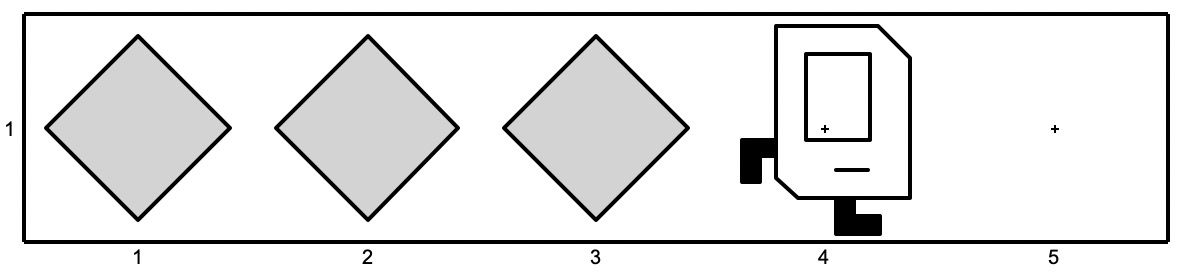
\includegraphics[scale=0.15]{images/ch04/mrofb/3rd_iter.jpg}
        \caption{တတိယ တစ်ကျော့ပြီး}  
        \label{fig:mrofb_recur4}  
    \end{subfigure}
    \begin{subfigure}[t]{{\figpctw}\textwidth}
        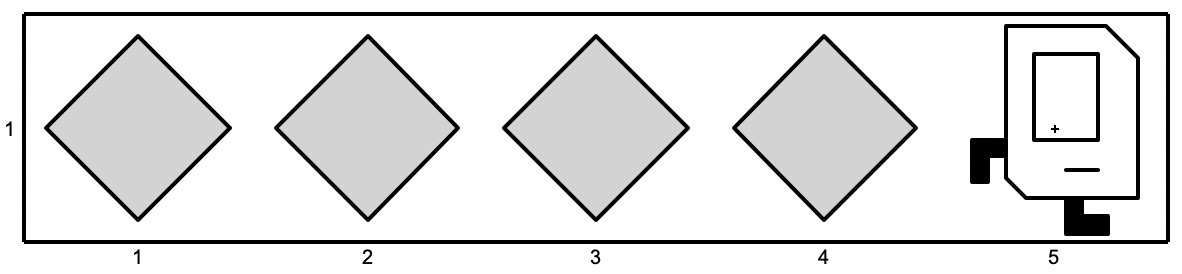
\includegraphics[scale=0.15]{images/ch04/mrofb/4th_iter.jpg}
        \caption{စတုတ္ထမြောက် ကျော့ပြီး}  
        \label{fig:mrofb_recur5}  
    \end{subfigure}
    \begin{subfigure}[t]{{\figpctw}\textwidth}
        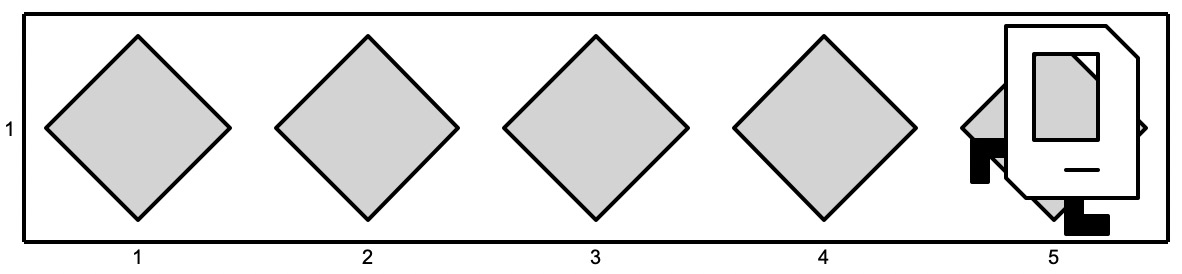
\includegraphics[scale=0.15]{images/ch04/mrofb/after.jpg}
        \caption{နောက်ဆုံး \fCptCodeBf{putBeeper} လုပ်ပြီး}    
        \label{fig:mrofb_recur6}
    \end{subfigure}
    \caption{}
    \label{fig:mrofb_recur}
\end{figure}


%
\setlength{\fboxsep}{0pt}
\begin{minted}[frame=\mintframe, framerule=\mintrule,framesep= \mintsep, xleftmargin=\xlftmargin
    , bgcolor=mintbgcolor,rulecolor=mintrulecolor
    , python3=true,escapeinside=ßß]{python}
def make_beeper_row():
    if front_is_clear():ß\tikzmark{xx2}ß
        put_beeper()
        move()
        make_beeper_row()ß\tikzmark{xx3}ß
    else:
        put_beeper()ß\tikzmark{xx4}ß

make_beeper_row()ß\tikzmark{xx1}ß
\end{minted}
%
\begin{tikzpicture}[
  remember picture,
  overlay,
  annotation/.style={
    inner sep=0pt,
    outer sep=0pt,
    outer xsep=0mm,
    fill=yellow!80!black,
    text width=5cm
  },
  >={Stealth[inset=0pt, angle=30:7pt]}
]
\draw[->, thick] ([yshift=0ex] pic cs:xx1) -- ++(3,0) |- ([yshift=1.4ex]pic cs:xx2);%
\draw[->, thin,blue] ([yshift=0ex] pic cs:xx3) -- ++(1,0) |- ([yshift=0.5ex] pic cs:xx2);%
\draw[->, thin,blue] ([yshift=1.2ex] pic cs:xx3) -- ++(.7,0) |- ([yshift=-.4ex] pic cs:xx2);%
\draw[->, thin,red] ([yshift=0.5ex] pic cs:xx4) -- ++(.7,0) |- ([yshift=1.2ex] pic cs:xx1);%
\end{tikzpicture}%
\btwntikzannoandpar

ရီကားဆစ်ဖ်ကောလ် ဖြစ်တာကို စိတ်ကူးပုံဖော်ကြည့်ဖို့ ပြထားတာပါ။ အပြင်ဆုံး မြှားအနက်က ကန\allowbreak ဦး ဖန်ရှင်ကောလ် စတင်တာဖြစ်‌ပေါ်တာကို ဖော်ပြတယ်။ ရီကားဆစ်ဖ်ကောလ် မဟုတ်သေးဘူး။ မြှားအပြာက ရီကားဆစ်ဖ်ကောလ်ကြောင့် ဖန်ရှင်အစ ပြန်ရောက်သွားတာကို ပြတယ်။ ပထမနဲ့ ဒုတိယ ရီကားဆစ်ဖ်ကောလ် နှစ်ခုအတွက်ပြထားတာပါ။ ရှေ့က ဥပမာအတွက် မြှားအပြာ လေးခု ရှိရမှာပါ (ရီကားဆစ်ဖ်ကောလ် လေးကြိမ်အတွက်)။  မြှားအပြာ နောက်ထပ် နှစ်ခုရှိတယ် မှတ်ယူပါ (ပုံမှာထပ်ထည့်ရင် ကြပ်ညပ်ပြီး ကြည့်ရရှုပ်လို့ မဆွဲပြတာ)။ လေးကြိမ်မြောက်မှာ ရီကားဆစ်ဖ်ကောလ် ထပ်မဖြစ်တော့ဘူး (\fCode{if} အပိုင်းကို မလုပ်တော့တဲ့အတွက်)။ ဘိပါချပြီး ဖန်ရှင်ကောလ် စခဲ့တဲ့နေရာကို ပြန်ရောက် သွားမယ် (မြှားအနီ)။ ဘယ်လို ပြန်ရောက်သွားတာလဲ ဆက်ကြည့်ရအောင်။

\subsection*{နောက်ဆုံး ရီကားဆစ်ဖ်ကောလ်မှ ပြန်လာခြင်း}
နောက်ဆုံး ရီကားဆစ်ဖ်ကောလ်ကနေ မူလ ဖန်ရှင်ခေါ်ခဲ့တဲ့ နေရာကို ဘယ်လိုပြန်ရောက်သွားတာလဲ။ ဒီကိစ္စနားလည်ဖို့ ဖန်ရှင် \fEnEmp{return} ပြန်ခြင်းအကြောင်း အရင်ကြည့်ရပါမယ်။ ဖန်ရှင်ကောလ် လုပ်ဆောင်တဲ့အခါ အဲဒီဖန်ရှင်နဲ့ သက်ဆိုင်တဲ့ ဘလောက်ဆီကို ခုန်ကျော် ရောက်ရှိသွားမှာပါ။ ဖန်ရှင်ဘလောက်ကို လုပ်ဆောင်ပြီး ခေါ်ခဲ့တဲ့ နေရာကို ပြန်လည်ရောက်ရှိသွားမှာ ဖြစ်တယ်။ ဒီဖြစ်စဉ်ကို ဖန်ရှင် \fEn{return} ပြန်တယ်လို့ ပြောပါတယ်။
%
\setlength{\fboxsep}{0pt}
\begin{minted}[frame=\mintframe, framerule=\mintrule,framesep= \mintsep, xleftmargin=\xlftmargin
    , bgcolor=mintbgcolor,rulecolor=mintrulecolor
    , python3=true,escapeinside=ßß]{python}
def main():
    turn_right()ß\tikzmark{a}ß
    move()
    turn_right()
    move()

def turn_right():
    turn_left()ß\tikzmark{b}ß
    turn_left()
    turn_left()ß\tikzmark{c}ß
\end{minted}
\begin{tikzpicture}[
  remember picture,
  overlay,
  annotation/.style={
    inner sep=0pt,
    outer sep=0pt,
    outer xsep=1mm,
    fill=yellow!80!black,
    text width=5cm
  },
  >={Stealth[inset=0pt, angle=30:7pt]}
]
\draw[->, thin] (pic cs:a)  ++(0,1.2ex) -- ++(1,0) |- ([yshift=0.5ex] pic cs:b);
\draw[->, thin, red] (pic cs:c)  ++(0,.5ex) -- ++(2,0) |- (pic cs:a);
%\draw[->] (pic cs:aa)  ++(0,1ex) -- ++(2.5,0) |- ([shift={(0,-0.5ex)}] pic cs:b) ;
\end{tikzpicture}%
ပထမ \fCode{turn\_right} ကောလ် လုပ်ဆောင်တဲ့အခါ ကောလ်လုပ်တဲ့ နေရာကနေ \fCode{turn\_right} ဖန်ရှင်ထဲကို \fEn{jump} လုပ်ပြီး ရောက်သွားတယ်။ မြှားအနက်နဲ့ ပြထားတယ်။ ဖန်ရှင်ဘလောက် လုပ်ဆောင်ပြီးတဲ့အခါ ခေါ်ခဲ့တဲ့နေရာ \fCode{main} ဖန်ရှင်ထဲ ပြန်ရောက်သွားတယ် (မြှားအနီ)။ ဒုတိယ \fCode{turn\_right} လည်း ထိုနည်းတူစွာပဲ ဖြစ်ပါတယ်။


%
\setlength{\fboxsep}{0pt}
\begin{minted}[frame=\mintframe, framerule=\mintrule,framesep= \mintsep, xleftmargin=\xlftmargin
    , bgcolor=mintbgcolor,rulecolor=mintrulecolor
    , python3=true,escapeinside=ßß]{python}
def main():
    turn_right()
    move()
    turn_right()ß\tikzmark{aa}ß
    move()

def turn_right():
    turn_left()ß\tikzmark{bb}ß
    turn_left()
    turn_left()ß\tikzmark{cc}ß
\end{minted}
\begin{tikzpicture}[
  remember picture,
  overlay,
  annotation/.style={
    inner sep=0pt,
    outer sep=0pt,
    outer xsep=1mm,
    fill=yellow!80!black,
    text width=5cm
  },
  >={Stealth[inset=0pt, angle=30:7pt]}
]
\draw[->, thin] (pic cs:aa)  ++(0,1.2ex) -- ++(1,0) |- ([yshift=0.5ex] pic cs:bb);
\draw[->, thin, red] (pic cs:cc)  ++(0,.5ex) -- ++(2,0) |- (pic cs:aa);
\end{tikzpicture}
\btwntikzannoandpar

နှစ်ဆင့်၊ သုံးဆင့် ဖန်ရှင်ကောလ်တွေမှာလည်း ဒီသဘောတရား အတိုင်းပါပဲ။ အောက်ဖော်ပြပါ ပရိုဂရမ်ကုဒ်ကို ကြည့်ပါ။ \fCode{main} ဖန်ရှင်ထဲကနေ \fCode{do\_tricks} ဆီကို ရောက်သွားမယ်။ \fCode{do\_tricks} ထဲကနေ \fCode{put\_two} ထဲကို ရောက်သွားမယ်။ 
%
\setlength{\fboxsep}{0pt}
\begin{minted}[frame=\mintframe, framerule=\mintrule,framesep= \mintsep, xleftmargin=\xlftmargin
    , bgcolor=mintbgcolor,rulecolor=mintrulecolor
    , python3=true,escapeinside=ßß]{python}
def main():
    do_tricks()ß\tikzmark{a2}ß
    move()

def do_tricks():
    move()ß\tikzmark{b2}ß
    put_two()ß\tikzmark{c2}ß
    turn_left()
    move()ß\tikzmark{d2}ß

def put_two():
    put_beeper()ß\tikzmark{e2}ß
    put_beeper()ß\tikzmark{f2}ß
\end{minted}
\begin{tikzpicture}[
  remember picture,
  overlay,
  annotation/.style={
    inner sep=0pt,
    outer sep=0pt,
    outer xsep=1mm,
    fill=yellow!80!black,
    text width=5cm
  },
  >={Stealth[inset=0pt, angle=30:7pt]}
]
\draw[->, thin] (pic cs:a2)  ++(0,1.2ex) -- ++(1,0) |- ([yshift=0.5ex] pic cs:b2);
\draw[->, thin] (pic cs:c2)  ++(0,1.2ex) -- ++(1,0) |- ([yshift=0.5ex] pic cs:e2);
\draw[->, thin, red] (pic cs:f2)  ++(0,.5ex) -- ++(0.7,0) |- (pic cs:c2);
\draw[->, thin, red] (pic cs:d2)  ++(0,.5ex) -- ++(2.1,0) |- (pic cs:a2);
\end{tikzpicture}%
\fCode{put\_two} ပြီးသွားတဲ့အခါ \fCode{do\_tricks} ထဲ ပြန်ရောက်သွားမယ်။ \fCode{turn\_left}\fEn{,} \fCode{move} ဆက်လုပ်ပြီး \fCode{do\_tricks} ခေါ်ခဲ့တဲ့နေရာ \fCode{main} ထဲ ပြန်ရောက်သွားမယ်။ နောက်ဆုံး \fCode{main} ထဲက \fCode{move}  ကို ဆက်လုပ်ပါတယ်။

ဖန်ရှင် အဆင့်ဆင့် ခေါ်ထားတဲ့အခါ နောက်ဆုံးခေါ်တဲ့ ဖန်ရှင်က အရင်ဆုံး \fEn{return} ပြန်ပါတယ်။ \fCode{main} ကနေ \fCode{do\_tricks} ကိုခေါ်၊ \fCode{do\_tricks} ကနေ \fCode{put\_two} ကိုခေါ်ထားရင် \fCode{put\_two} ကနေ \fCode{do\_tricks} ဆီကို အရင် \fEn{return} ပြန်တယ်။ ပြီးတော့မှ \fCode{do\_tricks} ကနေ \fCode{main} ကို ပြန်ရောက်မှာပါ။ ဒီသဘောအရ \fCode{put\_two} \fEn{return} မပြန်မချင်း \fCode{do\_tricks} ဖန်ရှင်မပြီးသေးဘူး။ \fCode{put\_two} ကနေပြန်လာပြီးမှ ကျန်တဲ့ \fCode{turn\_left}\fEn{,} \fCode{move} ဆက်လုပ်တယ်။ ပြီးတော့မှ \fCode{do\_tricks} ဖန်ရှင်က \fEn{return} ပြန်ပါတယ်။ 


ရီကားဆစ်ဖ် ဖန်ရှင်ကောလ်တွေ ဘယ်လို \fEn{return} ပြန်လဲ။ ရှေ့ကလို မြှားတွေနဲ့ ဆွဲပြလို့ ရပေမဲ့ ကြည့်ရတာ ရှုပ်ရှက်ခတ်နေမှာပါ။ အခုလို မြင်ကြည့်ရင် ပိုရှင်းပါတယ်။
%
\setlength{\fboxsep}{0pt}
\begin{minted}[frame=\mintframe, framerule=\mintrule,framesep= \mintsep, xleftmargin=\xlftmargin
    , bgcolor=mintbgcolor,rulecolor=mintrulecolor
    , python3=true,escapeinside=ßß]{python}
# ß\fEn{initial call}ß
make_beeper_row()ß\tikzmarknode{x1}ß
    # ß\fEn{1\textsuperscript{\fEn{st}} recur}ß
    make_beeper_row()ß\tikzmarknode{x2}ß
        # ß\fEn{2\textsuperscript{\fEn{nd}} recur}ß
        make_beeper_row()ß\tikzmarknode{x3}ß
            # ß\fEn{3\textsuperscript{\fEn{rd}} recur}ß
            make_beeper_row()ß\tikzmarknode{x4}ß
                # ß\fEn{4\textsuperscript{\fEn{th}} recur}ß
                make_beeper_row()ß\tikzmarknode{x5}ß
\end{minted}
\begin{tikzpicture}[
  remember picture,
  overlay,
  annotation/.style={
    inner sep=0pt,
    outer sep=0pt,
    outer xsep=1mm,
    fill=yellow!80!black,
    text width=5cm
  },
  >={Stealth[inset=0pt, angle=30:7pt]}
]
\draw[->, thin] (pic cs:x1)  ++(0,.3ex) .. controls ([xshift=1.1cm,yshift=-.11cm]pic cs:x1) and ([xshift=.5cm,yshift=.5cm]pic cs:x2) ..  ([yshift=1.2ex] pic cs:x2);
\draw[->, thin] (pic cs:x2)  ++(0,0ex) .. controls ([xshift=1.1cm,yshift=-.11cm]pic cs:x2) and ([xshift=.5cm,yshift=.5cm]pic cs:x3) ..  ([yshift=1.2ex] pic cs:x3);
\draw[->, thin] (pic cs:x3)  ++(0,0ex) .. controls ([xshift=1.1cm,yshift=-.11cm]pic cs:x3) and ([xshift=.5cm,yshift=.5cm]pic cs:x4) ..  ([yshift=1.2ex] pic cs:x4);
\draw[->, thin] (pic cs:x4)  ++(0,0ex) .. controls ([xshift=1.1cm,yshift=-.11cm]pic cs:x4) and ([xshift=.5cm,yshift=.5cm]pic cs:x5) ..  ([yshift=.7ex] pic cs:x5);
\draw[->, thin, red] (pic cs:x5)  ++(0,0ex) .. controls ([xshift=1.7cm,yshift=.4cm]pic cs:x5) and ([xshift=1cm,yshift=.2cm]pic cs:x4) ..  ([yshift=.5ex] pic cs:x4);
\draw[->, thin, red] (pic cs:x4)  ++(0,1ex) .. controls ([xshift=1.7cm,yshift=.4cm]pic cs:x4) and ([xshift=1cm,yshift=.2cm]pic cs:x3) ..  ([yshift=.5ex] pic cs:x3);
\draw[->, thin, red] (pic cs:x3)  ++(0,1ex) .. controls ([xshift=1.7cm,yshift=.4cm]pic cs:x3) and ([xshift=1cm,yshift=.2cm]pic cs:x2) ..  ([yshift=.5ex] pic cs:x2);
\draw[->, thin, red] (pic cs:x2)  ++(0,1ex) .. controls ([xshift=1.7cm,yshift=.4cm]pic cs:x2) and ([xshift=1cm,yshift=.2cm]pic cs:x1) ..  ([yshift=.7ex] pic cs:x1);
%([yshift=0.1em]a.north) to[bend left] ([yshift=0.1em]b.north);}
\end{tikzpicture}%
\btwntikzannoandpar

မြှားအနက်တွေက ဖန်ရှင်ကောလ်  တစ်ဆင့်ပြီးတစ်ဆင့် ဖြစ်တာကို ပြတာပါ။ အထက်မှအောက် အစီ\allowbreak အစဉ်အတိုင်း ဖြစ်ပါတယ်။ ‌လေးကြိမ်မြောက်မှာ နောက်ထပ် ရီကားဆစ်ဖ်ကောလ် ထပ်မဖြစ်တော့ဘဲ နောက်ဆုံး ရီကားဆစ်ဖ်ကောလ်က အရင်ဆုံး \fEn{return} စပြန်ပါတယ် (အောက်ဆုံး မြှားအနီနဲ့ ပြထား)။ ဒီအခါ တတိယ ရီကားဆစ်ဖ်ကောလ်ကို ပြန်ရောက်သွားမှာပါ။ ဒီအတိုင်း တစ်ဆင့်ပြီးတစ်ဆင့် အထက်ကို \fEn{return} ပြန်ပြီး နောက်ဆုံးမှာ ပထမဆုံး ခေါ်ခဲ့တဲ့နေရာ ပြန်ရောက်သွားမှာပါ။ (အခုပြထားတာကို တကယ့် \fEn{Python} ကုဒ် အနေနဲ့ မယူဆရပါ၊ ဖြစ်စဉ် နားလည်အောင် ပြခြင်းသာဖြစ်ပါတယ်)။

%
\setlength{\fboxsep}{0pt}
\begin{minted}[frame=\mintframe, framerule=\mintrule,framesep= \mintsep, xleftmargin=\xlftmargin
    , bgcolor=mintbgcolor,rulecolor=mintrulecolor
    , python3=true,escapeinside=ßß]{python}
from stanfordkarel import *

def main():
    make_beeper_row()

def make_beeper_row():
    if front_is_clear():
        put_beeper()
        move()
        make_beeper_row()
        turn_left()
        move()
    else:
        put_beeper()

if __name__ == "__main__":
    run_karel_program("make_beeper_row2")
\end{minted}
%

\fCode{make\_beeper\_row} ကိုပဲ နဲနဲပြင်ထားတဲ့ ဗားရှင်းပါ။ \fCode{if}  အပိုင်း ရီကားဆစ်ဖ်ကောလ်အပြီး  \fCode{turn\_\allowbreak left} နဲ့ \fCode{move} လုပ်ထားပါတယ်။  (နောက်ဆုံးတစ်ခုမှ လွဲ၍) ရီကားဆစ်ဖ်ကောလ်ဖြစ်တိုင်း  ၎င်းတို့ကို မလုပ်ဆောင်ရသေးဘဲ ကျန်ရှိနေမှာပါ။ ရီကားဆစ်ဖ်ကောလ် \fEn{return} ပြန်လာပြီးမှ ၎င်းတို့ကို ဆက်လုပ်မှာ ဖြစ်တယ်။ \fEn{return} ပြန်တဲ့ ဖြစ်စဉ်အရ အောက်ဆုံး \fCode{turn\_\allowbreak left} နဲ့ \fCode{move} ကို ပထမဆုံး လုပ်ဆောင်မှာ ဖြစ်တယ်။ အပေါ်ကို

%
\setlength{\fboxsep}{0pt}
\begin{minted}[frame=\mintframe, framerule=\mintrule,framesep= \mintsep, xleftmargin=\xlftmargin
    , bgcolor=mintbgcolor,rulecolor=mintrulecolor
    , python3=true,escapeinside=ßß]{python}
# ß\fEn{initial call}ß
make_beeper_row()ß\tikzmarknode{z1}ß
    # ß\fEn{1\textsuperscript{\fEn{st}} recur}ß
    make_beeper_row()ß\tikzmarknode{z2}ß
    turn_left()
    move()ß\tikzmarknode{z2a}ß
        # ß\fEn{2\textsuperscript{\fEn{nd}} recur}ß
        make_beeper_row()ß\tikzmarknode{z3}ß
        turn_left()
        move()ß\tikzmarknode{z3a}ß
            # ß\fEn{3\textsuperscript{\fEn{rd}} recur}ß
            make_beeper_row()ß\tikzmarknode{z4}ß
            turn_left()
            move()ß\tikzmarknode{z4a}ß
                # ß\fEn{4\textsuperscript{\fEn{th}} recur}ß
                make_beeper_row()ß\tikzmarknode{z5}ß
\end{minted}
\begin{tikzpicture}[
  remember picture,
  overlay,
  annotation/.style={
    inner sep=0pt,
    outer sep=0pt,
    outer xsep=1mm,
    fill=yellow!80!black,
    text width=5cm
  },
  >={Stealth[inset=0pt, angle=30:7pt]}
]
\draw[->, thin] (pic cs:z1)  ++(0,.3ex) .. controls ([xshift=1.1cm,yshift=-.11cm]pic cs:z1) and ([xshift=.5cm,yshift=.5cm]pic cs:z2) ..  ([yshift=1.2ex] pic cs:z2);
\draw[->, thin] (pic cs:z2)  ++(0,0ex) .. controls ([xshift=1.1cm,yshift=-.11cm]pic cs:z2) and ([xshift=.5cm,yshift=.5cm]pic cs:z3) ..  ([yshift=1.2ex] pic cs:z3);
\draw[->, thin] (pic cs:z3)  ++(0,0ex) .. controls ([xshift=1.1cm,yshift=-.11cm]pic cs:z3) and ([xshift=.5cm,yshift=.5cm]pic cs:z4) ..  ([yshift=1.2ex] pic cs:z4);
\draw[->, thin] (pic cs:z4)  ++(0,0ex) .. controls ([xshift=1.1cm,yshift=-.11cm]pic cs:z4) and ([xshift=.5cm,yshift=.5cm]pic cs:z5) ..  ([yshift=.7ex] pic cs:z5);
\draw[->, thin, red] (pic cs:z5)  ++(0,0ex) .. controls ([xshift=1.7cm,yshift=.4cm]pic cs:z5) and ([xshift=1cm,yshift=.2cm]pic cs:z4) ..  ([yshift=.5ex] pic cs:z4);
\draw[->, thin, red] (pic cs:z4a)  ++(0,.5ex) .. controls ([xshift=4.5cm,yshift=.7cm]pic cs:z4a) and ([xshift=1cm,yshift=.2cm]pic cs:z3) ..  ([yshift=.5ex] pic cs:z3);
\draw[->, thin, red] (pic cs:z3a)  ++(0,.5ex) .. controls ([xshift=4.5cm,yshift=.7cm]pic cs:z3a) and ([xshift=1cm,yshift=.2cm]pic cs:z2) ..  ([yshift=.5ex] pic cs:z2);
\draw[->, thin, red] (pic cs:z2a)  ++(0,.5ex) .. controls ([xshift=4.5cm,yshift=.7cm]pic cs:z2a) and ([xshift=1cm,yshift=.2cm]pic cs:z1) ..  ([yshift=.5ex] pic cs:z1);
%([yshift=0.1em]a.north) to[bend left] ([yshift=0.1em]b.north);}
\end{tikzpicture}



%
\setlength{\fboxsep}{0pt}
\begin{minted}[frame=\mintframe, framerule=\mintrule,framesep= \mintsep, xleftmargin=\xlftmargin
    , bgcolor=mintbgcolor,rulecolor=mintrulecolor
    , python3=true,escapeinside=ßß]{python}
def make_beeper_row():
    if front_is_clear():ß\tikzmark{s2}ß
        put_beeper()
        move()
        make_beeper_row()ß\tikzmark{s3}ß
        turn_left()
        move()ß\tikzmark{s3a}ß
    else:
        put_beeper()ß\tikzmark{s4}ß

# ß\fEn{initial call}ß
make_beeper_row()ß\tikzmark{s1}ß
\end{minted}
%
\begin{tikzpicture}[
  remember picture,
  overlay,
  annotation/.style={
    inner sep=0pt,
    outer sep=0pt,
    outer xsep=0mm,
    fill=yellow!80!black,
    text width=5cm
  },
  >={Stealth[inset=0pt, angle=30:7pt]}
]
\draw[->, thick] ([yshift=1.2ex] pic cs:s1) -- ++(3,0) |- ([yshift=1.4ex]pic cs:s2);%
\draw[->, thin,blue] ([yshift=.5ex] pic cs:s3) -- ++(1,0) |- ([yshift=0.5ex] pic cs:s2);%
\draw[->, thin,blue] ([yshift=1.4ex] pic cs:s3) -- ++(.7,0) |- ([yshift=-.4ex] pic cs:s2);%
\draw[->, thin,red] ([yshift=0.5ex] pic cs:s4) -- ++(1.5,0) |- ([yshift=-.4ex] pic cs:s3);%
\draw[->, thin,red] ([yshift=0.5ex] pic cs:s3a) -- ++(1.5,0) |- ([yshift=0ex] pic cs:s1);%
\end{tikzpicture}%
\btwntikzannoandpar